\documentclass[convert]{standalone}

\usepackage{tikz}
\usepackage{graphicx}
\pagestyle{empty}

% INT_AY22_L35-Fig03_Circle_polygon_points.png

\begin{document}
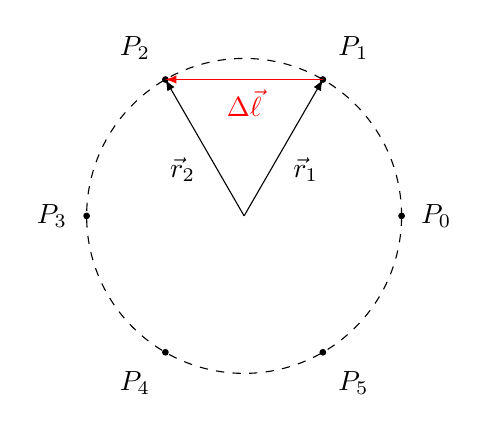
\begin{tikzpicture}[> = latex]

	% Definitions
	
	\def\R{2}		% Circle radius
	\def\N{5} 		% Number of polygonal sides - 1
	
	% Corners of polygon
	
	\foreach \Q in {0, 1, ..., \N}
		\filldraw ({360 * \Q / (\N + 1)} : 2) circle (1 pt) node [label = {360 * \Q / (\N + 1)}: {$P_\Q$}] {};
	
	% Position vectors
	
	\draw [->] (0, 0) -- node [below right] {${\vec r}_1$} (60 : \R);
	\draw [->] (0, 0) -- node [below left] {${\vec r}_2$} (120 : \R);
	
	% Position difference
	
	\draw [red, ->] (60 : \R) -- node [below] {$\Delta {\vec \ell}$} (120 : \R);

	% Actual circle
	
	\draw [dashed] (0, 0) circle (\R);

\end{tikzpicture}
\end{document}